\documentclass[12pt]{article}

\usepackage{amsmath}
\usepackage{amssymb}
\usepackage{amsthm}
\usepackage{fullpage}
\usepackage{makecell}
\usepackage{tabularx}

\usepackage[dvipsnames]{xcolor}
\usepackage{tikz,tkz-euclide}
\usetikzlibrary{decorations.pathreplacing}
\usetikzlibrary{quotes,angles,calc,intersections}
\usepackage{pgfplots}

\usepackage{titling}
\usepackage{pdfpages}
\usepackage{color}
\usepackage{hyperref}

\usepackage{common}
\usepackage{linear}

\begin{document}

\title{Mathematics of Images and Shapes Notes}
\author{Brendan Burkhart}
\maketitle

\tableofcontents
\newpage

\section{Mathematically Describing Images}

Traditionally, images have been modeled as graphs (or level sets) of continuous functions defined on a rectangular domain $D \subset \R^2$, and codomain $P \subset \R$. \[D = \left[0, R_1\right] \times \left[0, R_2\right] \subset \R^2\] \[P = \left[0, L\right] \subset \R\] \[f : D \to P\]

This definition is for grayscale (black and white), images, not color images. A value of $0$ would correspond to the color black, and $L$ to white, and everything in between would be various shades of gray.

To perform computational work with images, it is useful to discretize images. This can be done by sampling the functions at $(m, n)$ for all $m \in \{0, \ldots, M-1\}$ and $n \in \{0, \ldots, N-1\}$ where $M$ and $N$ are the number of pixels on the $y$-axis and $x$-axis respectively. $L$ is chosen to be $2^b-1$ where $b$ is the number of bits per pixel. We can then discretize the domain into $\mathbb{P} = \{0, \ldots, 2^b-1\}$. Discretized images are the graph of a discrete function $I: \mathbb{D} \to \mathbb{P}$, where $\mathbb{D} = \{0, \ldots, M-1\} \times \{0, \ldots, N-1\}$. This can be represented as an $M \times N$ matrix $I(i, j)$ where $(i, j) \in \mathbb{D}$.

Color images can be represented as three of these matrices (or a single three-dimensional matrix), each corresponding to one dimension of a color space, such as RGB or HSV.

\section{Point Operations}

\begin{defn}
    Given a mapping $T: \mathbb{P} \to \mathbb{P}$, a \emph{point operation} on an image $I: \mathbb{D} \to \mathbb{P}$ is defined as $J(i, j) = T(I(i, j))$ for all $(i, j) \in \mathbb{D}$.
\end{defn}

\begin{rmk}
    $J(i, j)$ depends only on $I(i, j)$, not on any other pixel.
\end{rmk}

\begin{defn}
    The \emph{Heaviside function} is $H: \R \to \R$, where $H(x) = \left\{
    \begin{array}{lr}
        1 & : x \geq 0 \\
        0 & : x < 0
    \end{array}\right.$
\end{defn}

For the following four examples, let $I = \begin{bmatrix}
    0 & 0 & 0\\ 255 & 255 & 0 \\ 255 & 0 & 100
\end{bmatrix}$, so $\mathbb{D} = \left[0, 2\right] \times \left[0, 2\right]$, and let $L = 2^8 = 256$ so $\mathbb{P} = \left[0, 256 - 1\right]$.

\begin{exmp}
    Identity: $T: r \mapsto r$, $J = \begin{bmatrix}
        0 & 0 & 0\\ 255 & 255 & 0 \\ 255 & 0 & 100
    \end{bmatrix}$.
\end{exmp}

\begin{exmp}
    Negative: $T: r \mapsto (L-1) - r$, $J = \begin{bmatrix}
        255 & 255 & 255 \\ 0 & 0 & 255 \\ 0 & 255 & 155
    \end{bmatrix}$.
\end{exmp}

\begin{exmp}
    B\&W: $T: r \mapsto (L-1)H(r - t)$ where $L \geq t \geq 0$. $J = \begin{bmatrix}
        0 & 0 & 0\\ 255 & 255 & 0 \\ 255 & 0 & 0
    \end{bmatrix}$.
\end{exmp}

\begin{figure}[ht!]
    \centering
    \begin{tikzpicture}[scale=1.0]
        \begin{axis}[
            axis x line=middle,
            axis y line=middle,
            ymin=0,ymax=256,ylabel=$y$,
            xmin=0,xmax=256,xlabel=$x$
            ]
        \addplot[domain=0:100, blue, ultra thick] {0};
        \addplot[domain=100:256, blue, ultra thick] {255};
        \addplot[color=blue,fill=white,only marks,mark=*] coordinates{(100,0)};
        \addplot[color=blue,only marks,mark=*] coordinates{(100,255)};
    \end{axis}
    \end{tikzpicture}
\caption{Graph of threshold function $(L-1)H(r - t)$ where $L = 256$ and $t = 100$.}
\label{fig:threshold}
\end{figure}

\begin{exmp}
    Gamma-correction: $T: r \mapsto (L-1)\left(\frac{r}{L-1}\right)^\gamma$ where $\gamma > 0$. When $\gamma > 1$ the image is darkened, when $\gamma < 1$ the image is brightened, and when $\gamma = 1$ the image is unchanged.
\end{exmp}

\begin{figure}[ht!]
    \centering
    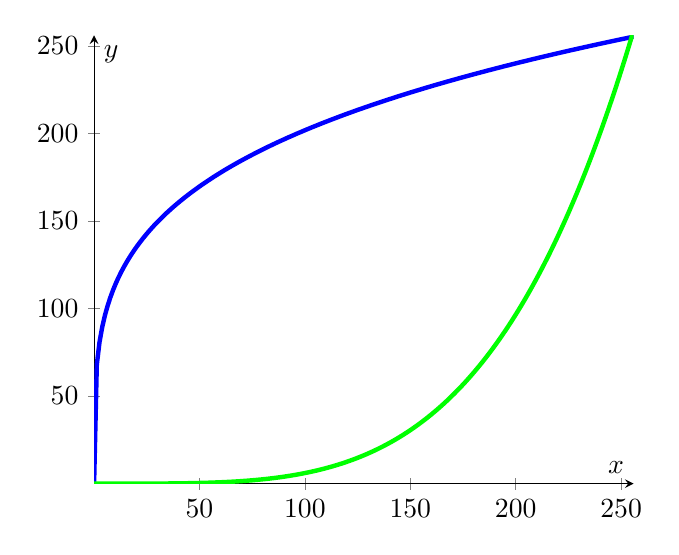
\begin{tikzpicture}[scale=01.0]
        \begin{axis}[
            axis x line=middle,
            axis y line=middle,
            ymin=0,ymax=256,ylabel=$y$,
            xmin=0,xmax=256,xlabel=$x$
            ]
        \addplot[domain=0:256, blue, ultra thick, samples=200] {255*(x/255)^0.25};
        \addplot[domain=0:256, green, ultra thick, samples=200] {255*(x/255)^4.0};
    \end{axis}
    \end{tikzpicture}
\caption{Graph of gamma function $(L-1)\left(\frac{r}{L-1}\right)^\gamma$ where $\gamma = 4$ (green) and $\gamma = \frac{1}{4}$ (blue).}
\label{fig:gamma}
\end{figure}

\begin{exmp}
    Contrast-enhancement: $T: r \mapsto c + c\sin\left(\frac{\pi(r-c)}{2c}\right)$ where $c = \frac{L - 1}{2}$. When $\gamma > 1$ the image is darkened, when $\gamma < 1$ the image is brightened, and when $\gamma = 1$ the image is unchanged.
\end{exmp}

\begin{figure}[ht!]
    \centering
    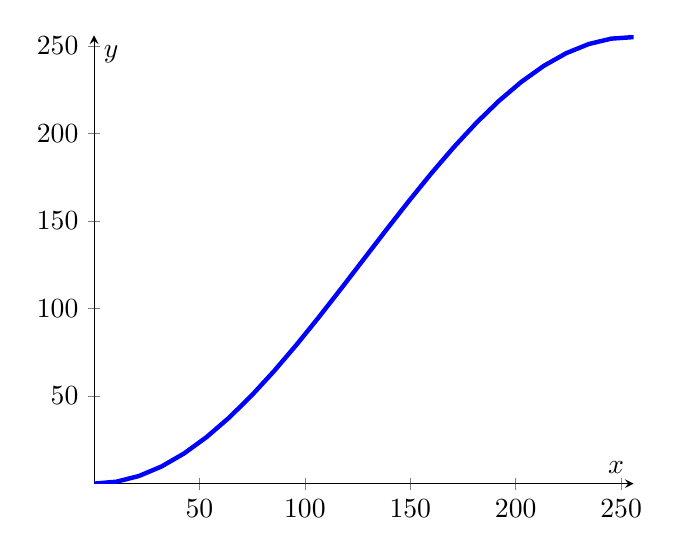
\begin{tikzpicture}[scale=01.0]
        \begin{axis}[
            axis x line=middle,
            axis y line=middle,
            ymin=0,ymax=256,ylabel=$y$,
            xmin=0,xmax=256,xlabel=$x$
            ]
        \addplot[domain=0:256, blue, ultra thick] {127.5 + 127.5*sin(deg(0.5*pi*(x - 127.5)/127.5))};
    \end{axis}
    \end{tikzpicture}
\caption{Graph of contrast enhancement $c + c\sin\left(\frac{\pi(r-c)}{2c}\right)$.}
\label{fig:contrast}
\end{figure}

\end{document}
